\documentclass{scrartcl} % scrartcl of scrreprt
% Include all project wide packages here.
\usepackage{fullpage}
\usepackage{polyglossia}
\setmainlanguage{dutch}
\usepackage{csquotes}
\usepackage{graphicx}
\usepackage{epstopdf}
\usepackage{pdfpages}
\usepackage{caption}
\usepackage[list=true]{subcaption}
\usepackage{float}
%\usepackage{mathtools}
\usepackage{standalone}
\usepackage{import}
\usepackage{tocloft}
\usepackage{wrapfig}
\usepackage{authblk}
\usepackage{array}
\usepackage{booktabs}
\usepackage[toc,page,title,titletoc]{appendix}
\usepackage{xunicode}
\usepackage{amsmath}
\usepackage{fontspec}
\usepackage{unicode-math}
\usepackage[
    backend=bibtexu,
	texencoding=utf8,
bibencoding=utf8,
    style=ieee,
    sortlocale=nl_NL,
    language=auto
]{biblatex}
\usepackage{listings}
\newcommand{\includecode}[3][c]{\lstinputlisting[caption=#2, escapechar=, style=#1]{#3}}
\newcommand{\superscript}[1]{\ensuremath{^{\textrm{#1}}}}
\newcommand{\subscript}[1]{\ensuremath{_{\textrm{#1}}}}


\newcommand{\chapternumber}{\thechapter}
\renewcommand{\appendixname}{Bijlage}
\renewcommand{\appendixtocname}{Bijlagen}
\renewcommand{\appendixpagename}{Bijlagen}

\usepackage[hidelinks]{hyperref} %<--------ALTIJD ALS LAATSTE

\renewcommand{\familydefault}{\sfdefault}

\setmainfont[Ligatures=TeX]{Myriad Pro}
\setmathfont{Asana Math}
\setmonofont{Lucida Console}

\usepackage{titlesec, blindtext, color}
\definecolor{gray75}{gray}{0.75}
\newcommand{\hsp}{\hspace{20pt}}
\titleformat{\chapter}[hang]{\Huge\bfseries}{\chapternumber\hsp\textcolor{gray75}{|}\hsp}{0pt}{\Huge\bfseries}
\renewcommand{\familydefault}{\sfdefault}
\renewcommand{\arraystretch}{1.2}
\setlength\parindent{0pt}

%For code listings
\definecolor{black}{rgb}{0,0,0}
\definecolor{browntags}{rgb}{0.65,0.1,0.1}
\definecolor{bluestrings}{rgb}{0,0,1}
\definecolor{graycomments}{rgb}{0.4,0.4,0.4}
\definecolor{redkeywords}{rgb}{1,0,0}
\definecolor{bluekeywords}{rgb}{0.13,0.13,0.8}
\definecolor{greencomments}{rgb}{0,0.5,0}
\definecolor{redstrings}{rgb}{0.9,0,0}
\definecolor{purpleidentifiers}{rgb}{0.01,0,0.01}


\lstdefinestyle{csharp}{
language=[Sharp]C,
showspaces=false,
showtabs=false,
breaklines=true,
showstringspaces=false,
breakatwhitespace=true,
escapeinside={(*@}{@*)},
columns=fullflexible,
commentstyle=\color{greencomments},
keywordstyle=\color{bluekeywords}\bfseries,
stringstyle=\color{redstrings},
identifierstyle=\color{purpleidentifiers},
basicstyle=\ttfamily\small}

\lstdefinestyle{c}{
language=C,
showspaces=false,
showtabs=false,
breaklines=true,
showstringspaces=false,
breakatwhitespace=true,
escapeinside={(*@}{@*)},
columns=fullflexible,
commentstyle=\color{greencomments},
keywordstyle=\color{bluekeywords}\bfseries,
stringstyle=\color{bluestrings},
identifierstyle=\color{purpleidentifiers}
}

\lstdefinestyle{vhdl}{
language=VHDL,
showspaces=false,
showtabs=false,
breaklines=true,
showstringspaces=false,
breakatwhitespace=true,
escapeinside={(*@}{@*)},
columns=fullflexible,
commentstyle=\color{greencomments},
keywordstyle=\color{bluekeywords}\bfseries,
stringstyle=\color{redstrings},
identifierstyle=\color{purpleidentifiers}
}

\lstdefinestyle{xaml}{
language=XML,
showspaces=false,
showtabs=false,
breaklines=true,
showstringspaces=false,
breakatwhitespace=true,
escapeinside={(*@}{@*)},
columns=fullflexible,
commentstyle=\color{greencomments},
keywordstyle=\color{redkeywords},
stringstyle=\color{bluestrings},
tagstyle=\color{browntags},
morestring=[b]",
  morecomment=[s]{<?}{?>},
  morekeywords={xmlns,version,typex:AsyncRecords,x:Arguments,x:Boolean,x:Byte,x:Char,x:Class,x:ClassAttributes,x:ClassModifier,x:Code,x:ConnectionId,x:Decimal,x:Double,x:FactoryMethod,x:FieldModifier,x:Int16,x:Int32,x:Int64,x:Key,x:Members,x:Name,x:Object,x:Property,x:Shared,x:Single,x:String,x:Subclass,x:SynchronousMode,x:TimeSpan,x:TypeArguments,x:Uid,x:Uri,x:XData,Grid.Column,Grid.ColumnSpan,Click,ClipToBounds,Content,DropDownOpened,FontSize,Foreground,Header,Height,HorizontalAlignment,HorizontalContentAlignment,IsCancel,IsDefault,IsEnabled,IsSelected,Margin,MinHeight,MinWidth,Padding,SnapsToDevicePixels,Target,TextWrapping,Title,VerticalAlignment,VerticalContentAlignment,Width,WindowStartupLocation,Binding,Mode,OneWay,xmlns:x}
}

%defaults
\lstset{
basicstyle=\ttfamily\small,
extendedchars=false,
numbers=left,
numberstyle=\ttfamily\tiny,
stepnumber=1,
tabsize=4,
numbersep=5pt
}
\addbibresource{../../library/bibliography.bib}

\author{Peter Stijnman}
\title{EPO3: Eindrapport - Resultaten}

\begin{document}
\chapter{Resultaten}
\label{ch:resultaten}


Nadat alle code geschreven, gesynthetyseerd en getest was is er gekeken na het totale eindresultaat van het project. De uiteindelijke layout van de chip samen met het aantal gebruikte transistoren en de bijbehorende efficiëntie. Ook is er getest met een FPGA.

\section{VHDL code}

Als eerste is de VHDL-code getest met een wave die klopte volgens de verwachting, we hebben hier helaas niet heel veel tijd voor gehad om uitvoerig te testen. Er zijn namelijk veel verschillende soort opdrachten die onze GPU kan uitvoeren en om voor elke situatie te simuleren was geen tijd meer voor. Het resultaat van de test is hieronder te zien.

\begin{figure}[H]
	\centering
	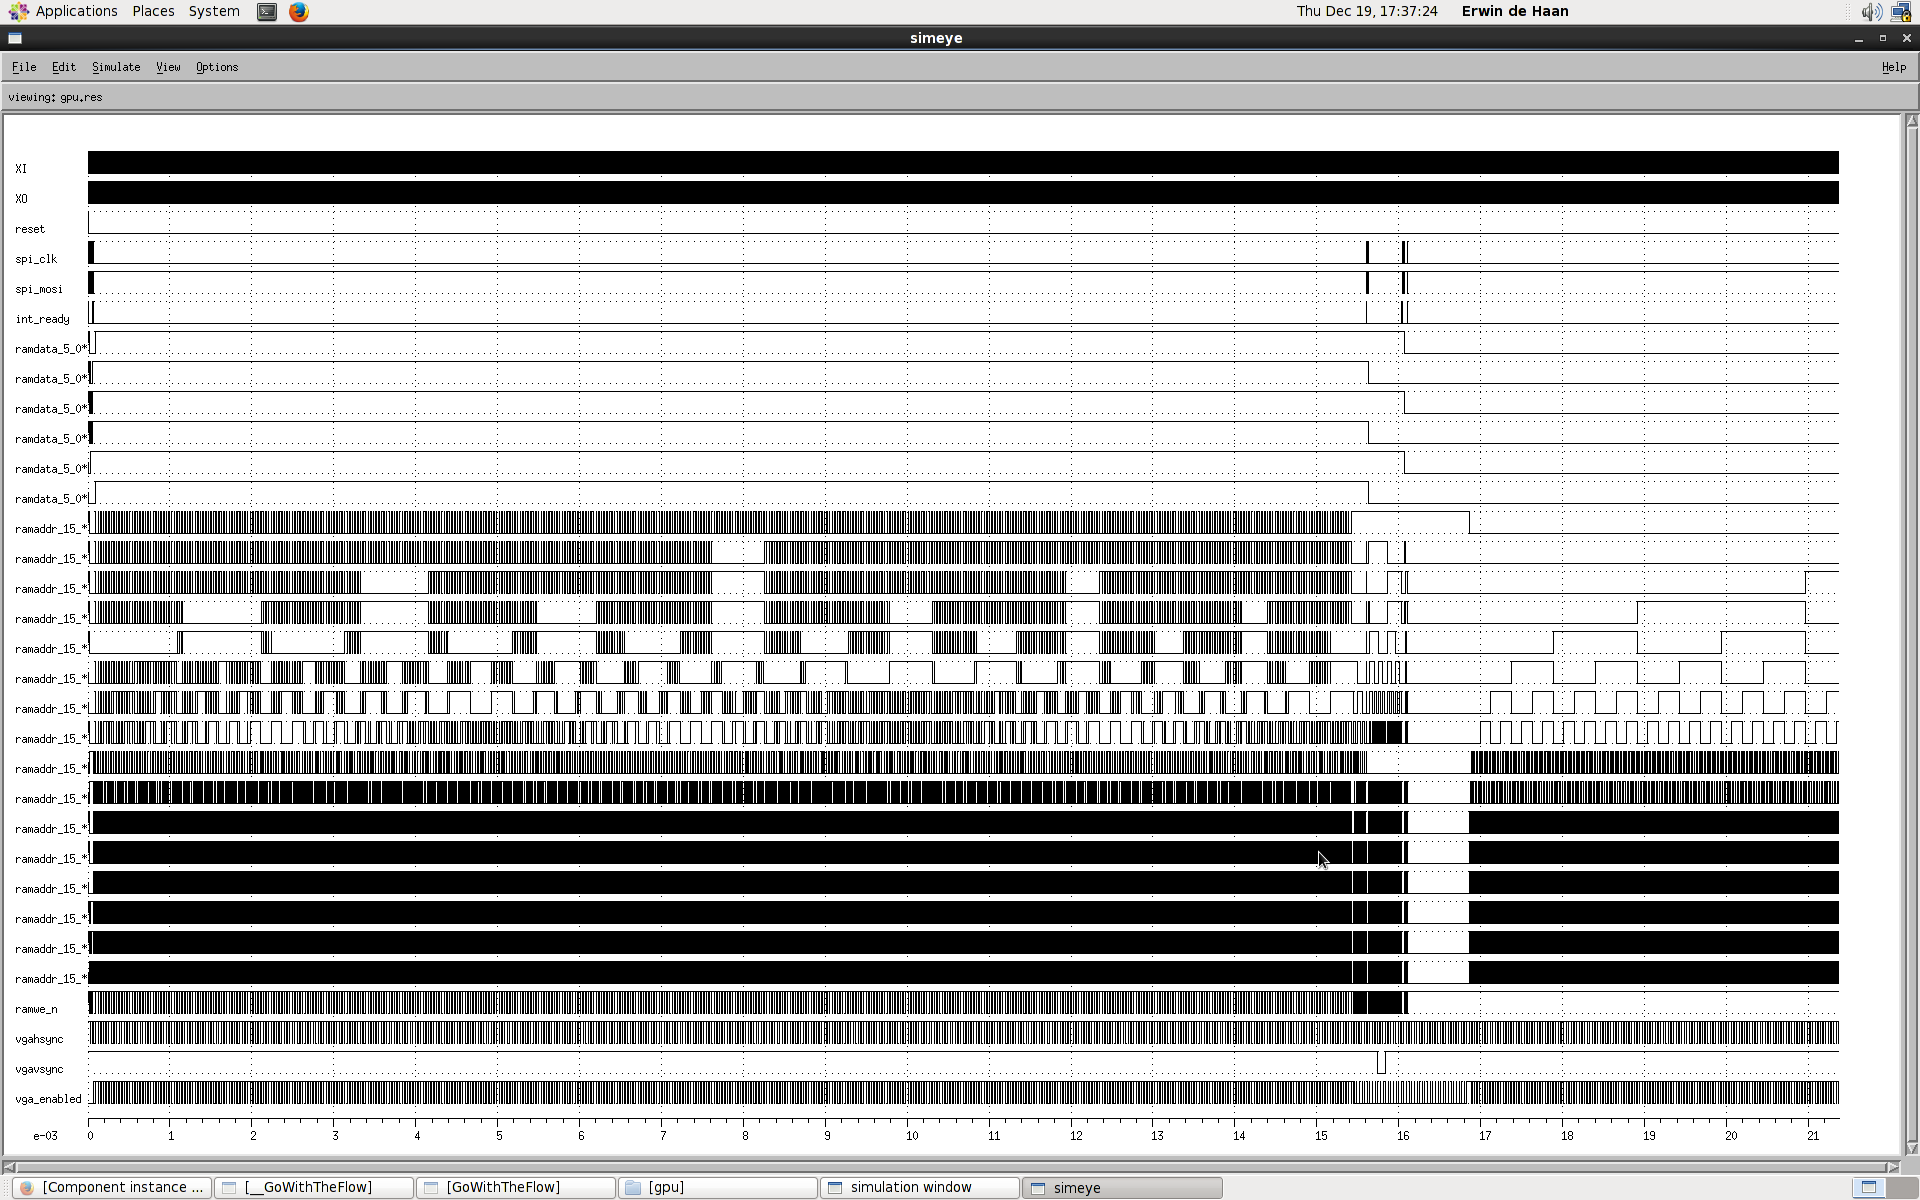
\includegraphics[width=0.8\textwidth]{layout_sls_wave}
	\caption{Resultaat van VHDL-code test}
\end{figure}



\section{FPGA test}

Nadat de VHDL-code getest was hebben we het ontwerp getest met behulp van een FPGA, op deze manier kregen werd er op een monitor een beeld geprojecteerd en kon er daadwerkelijk gezegd worden of de GPU de opdrachten goed uitvoerde. Ook konden we nu testen met de AVR en het externe RAM. Op deze manier kregen we meer inzicht in het totale ontwerp van de chip en konden er nog gemakkelijk veranderingen gemaakt worden in het ontwerp van de chip en de code in de AVR.\\  Het is lastig om een duidelijk resultaat te laten zien van de FPGA test aangezien het een bewegend beeld is, maar toch hebben we er een screenshot van gemaakt.

\begin{figure}[H]
	\centering
	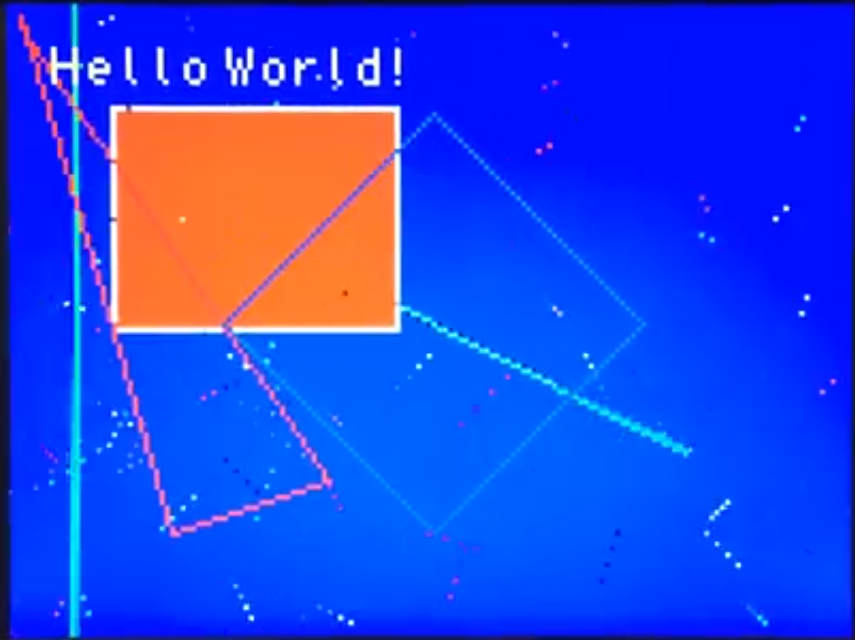
\includegraphics[width=0.8\textwidth]{FPGAtest}
	\caption{Resultaat van VHDL-code test}
\end{figure}

In dit frame is te zien dat onze GPU instaat is om pixels,rechthoeken,lijnen en zelfs sprite te kunnen tekenen.


\section{Synthese}

Als laatste was er het synthetyseren van het totale ontwerp. Tijdens dit process kwamen we er achter dat de module Draw Line te groot was voor de chip, inprincipe zou alles gemakkelijk passen op de chip alleen zou er dan niks geroute kunnen worden. We hebben er toen dus voor gekozen om deze module eruit te halen. Deze module was wel succesvol getest op de FPGA. Hieronder is de uiteindelijk layout van ons ontwerp te zien.


\begin{figure}[H]
	\centering
	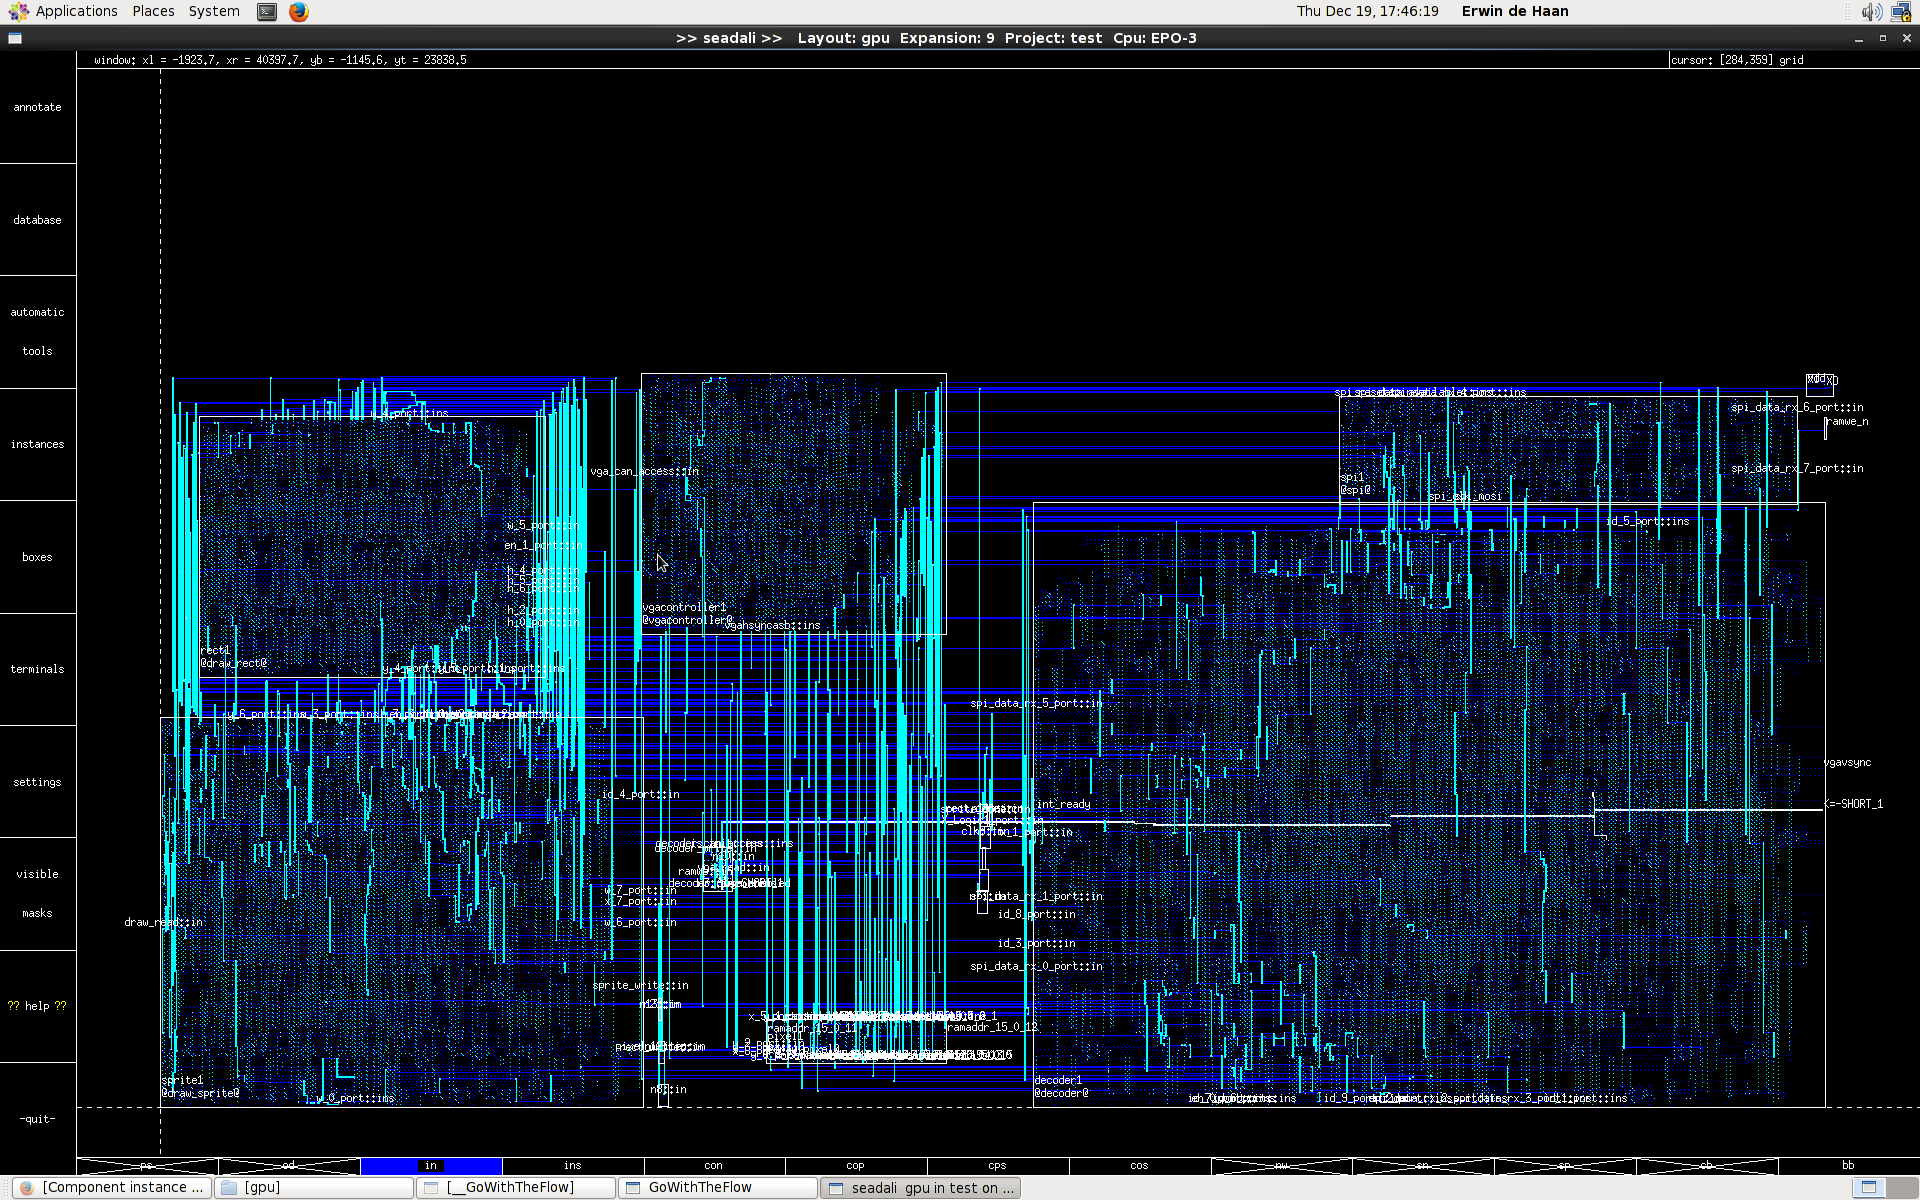
\includegraphics[width=0.8\textwidth]{layout}
	\caption{Resultaat van VHDL-code test}
\end{figure}

Het aantal gebruikte transistoren is 71854/16146, dit resulteert in een efficiëntie van 22,47\%. Het percentage had een stuk hoger kunnen liggen als we toch de module Draw Line hadden kunnen implementeren op de chip, deze module was namelijk ongeveer 25000 transistoren hiermee zou onze efficiëntie boven de 50\% uitkomen. Helaas was dit niet meer te routen met de programma's en technologie die wij tot onze beschikking hadden.






\end{document}
